\documentclass[conference]{IEEEtran}
\IEEEoverridecommandlockouts
 
\usepackage{amssymb}
\usepackage[table]{xcolor}
\usepackage{xspace}
\usepackage{booktabs}
\usepackage{amsmath}
\usepackage{graphicx}
\usepackage{algorithm}
\usepackage{algpseudocode}
\usepackage{float}
\usepackage{cite}
\usepackage{subcaption}
\usepackage{makecell}
\usepackage{xurl}
\usepackage{tikz}
\usetikzlibrary{arrows.meta, positioning, patterns, calc}
 
% ---- Macros ----
\newcommand{\smarm}{SMARM\xspace}
\newcommand{\tdis}{$t_{\mathrm{disabled}}$\xspace}
\newcommand{\FAR}{FAR\xspace}
 
\begin{document}
 
\title{.........}
 
% DOUBLE-BLIND: comment out \author block before submitting to ICSEC
\author{
  \IEEEauthorblockN{Amarin Laohajirapan, Norrathep Rattanavipanon}
  \IEEEauthorblockA{College of Computing,
    Prince of Songkla University, Phuket Campus, Thailand \\
    norrathep.r@psu.ac.th}
}
 
\maketitle
 
% ================================================================
\begin{abstract}
Remote attestation (RA) is a fundamental security primitive for
detecting software compromise on resource-constrained IoT devices.
SMARM reduces the non-interruptible period of traditional RA from the
entire memory scan down to a single block measurement, enabling
coexistence with real-time workloads. However, we show that SMARM
still violates real-time deadlines when block sizes exceed 1024~bytes
on commodity ARM Cortex-M33 hardware, because interrupts remain
disabled for the entire duration of each block's SHA-256 hash
computation.
We propose \emph{Atomic Copy}, an enhancement that shifts the
interrupt-disabled window from cryptographic hashing to memory copy.
Since memory copy on Cortex-M33 runs approximately $15\times$ faster
than SHA-256, this change reduces the non-interruptibility period
by 15--71$\times$ across all evaluated block sizes. We implement
Atomic Copy within a TrustZone-M-based SMARM realization running
FreeRTOS on the STM32L552ZE platform and evaluate it using the
Frequency Accuracy Ratio (FAR) metric. Our results show that Atomic
Copy restores FAR~$\approx 1.0$ across all evaluated block sizes up
to 4096~bytes, completely eliminating the real-time bottleneck of
SMARM while preserving its original security guarantees.
\end{abstract}
 
\begin{IEEEkeywords}
Remote attestation, IoT security, TrustZone-M, RTOS, real-time systems,
shuffled measurement, interrupt latency
\end{IEEEkeywords}

% ================================================================
\section{Introduction}
\label{sec:intro}
 
IoT and embedded devices are increasingly deployed in safety-critical
environments --- autonomous vehicles, medical monitors, industrial
controllers --- where both software integrity and real-time
availability are non-negotiable requirements. Remote attestation (RA)
enables a remote verifier to detect software compromise on such
devices, but traditional
RA~\cite{eldefrawy2012smart,nunes2019vrased,eldefrawy2017hydra}
requires interrupts to remain disabled for the entire memory
measurement. On a resource-constrained Cortex-M33 device, this window
can exceed 450~ms~\cite{nunes2019vrased}, blocking time-sensitive
tasks from executing and causing deadline violations.
 
SMARM~\cite{carpent2018smarm} addresses this by measuring memory
blocks in a secret shuffled order and re-enabling interrupts after
each block. This limits the non-interruptible window to a single block
measurement rather than the entire memory region. However, SMARM was
designed for the seL4 microkernel and has neither been ported to
commodity RTOS platforms nor evaluated under real-time workloads.
 
In this paper, we make two contributions. First, we present the first
port and evaluation of SMARM on FreeRTOS and Zephyr using ARM
TrustZone-M as the trust anchor. We show that SMARM fails to maintain
FAR~$\approx 1.0$ at block sizes $B \geq 2048$~bytes, where \tdis
exceeds the period of common real-time tasks. Second, we propose
\emph{Atomic Copy}, which shifts the atomic operation from SHA-256
hashing to memory copy, reducing \tdis by 15--71$\times$ and
restoring FAR~$\approx 1.0$ at all evaluated block sizes while
preserving SMARM's security guarantees (S1)--(S3).
 
A companion extended version studying secure-storage reduction
(SMARM+PRNG and SMARM+FPE variants), formal security proofs, and
energy consumption measurements is under preparation for journal
submission.
% ================================================================

\section{Background}
\label{sec:background}
 
\subsection{Remote Attestation and the Atomicity Problem}
 
In a typical RA protocol, the verifier sends a fresh challenge to the
prover (IoT device), which computes a cryptographic measurement
(e.g., HMAC-SHA256) over its program memory and returns it as
attestation evidence. To prevent \emph{roving malware} that relocates
itself to evade detection, traditional
RA~\cite{eldefrawy2012smart,nunes2019vrased} requires this computation
to execute atomically with interrupts fully disabled. The resulting
non-interruptible window scales with memory size: VRASED reports up to
450~ms on comparable hardware~\cite{nunes2019vrased}, during which all
real-time tasks are blocked.
 
Table~\ref{tab:ra_comparison} summarizes how traditional RA, SMARM,
and our Atomic Copy compare. Traditional RA provides strong security
but is incompatible with real-time workloads. SMARM reduces the
non-interruptible window but retains per-block hashing atomicity.
Atomic Copy further decouples the atomic operation from hashing,
achieving real-time compatibility at all block sizes.
 
\begin{table}[!ht]
  \centering
  \caption{Comparison of attestation approaches for real-time
           IoT devices.}
  \label{tab:ra_comparison}
  \renewcommand{\arraystretch}{1.1}
  \small
  \setlength{\tabcolsep}{3pt}
  \begin{tabular}{p{1.6cm}cccp{1.4cm}}
    \toprule
    \textbf{Approach} &
    \textbf{RT-safe} &
    \makecell{\textbf{No} \\ \textbf{extra HW}} &
    \makecell{\textbf{Atomic} \\ \textbf{window}} &
    \textbf{RTOS} \\
    \midrule
    Traditional RA~\cite{eldefrawy2012smart} &
      \texttimes & \checkmark & Full scan & \texttimes \\
    SMARM~\cite{carpent2018smarm} &
      Partial & \checkmark & Per-block hash & \texttimes \\
    \textbf{Atomic Copy (ours)} &
      \checkmark & \checkmark & Per-block copy & \checkmark \\
    \bottomrule
  \end{tabular}
\end{table}
 
\subsection{SMARM: Shuffled Measurements Against Roving Malware}
 
SMARM~\cite{carpent2018smarm} derives a one-time permutation $\sigma$
over memory block indices from a shared secret key $k$ and verifier
challenge $\mathit{chal}$:
\[
  \sigma = \mathrm{FisherYates}(\mathrm{Hash}(\mathit{chal}, k),\;
           [0,\ldots,n{-}1]).
\]
The prover measures each block $M_{\sigma(i)}$ in this shuffled order,
disabling interrupts only during the HMAC update for each block. Since
roving malware cannot predict $\sigma$, its probability of evading
detection is bounded by $(1-1/n)^n \approx e^{-1} \approx 37\%$ per
round; multiple rounds reduce this further.
 
SMARM requires three security properties: \textbf{(S1) Controlled
Execution} --- the attestation service is invocable only through
defined entry/exit points and interrupts may only be re-enabled
between block measurements; \textbf{(S2) Key Secrecy} --- $k$ is
inaccessible to untrusted software; \textbf{(S3) Private Measurement
Order} --- $\sigma$ is stored in memory inaccessible to KFV malware.
 
\subsection{Porting SMARM to FreeRTOS + TrustZone-M}
\label{sec:port}
 
The original SMARM prototype relied on the seL4 microkernel's formally
verified isolation to protect $k$ and $\sigma$~\cite{klein2009sel4}.
A naive replacement of seL4 with a commodity RTOS is insufficient: in
vanilla FreeRTOS, all tasks execute at the same privilege level,
allowing any compromised task to read or modify $k$ and $\sigma$,
breaking (S2) and (S3). Even RTOSes with optional memory isolation
have been shown to contain exploitable
vulnerabilities~\cite{freertos_cve,zephyr_cve}.
 
We implement SMARM on the STM32L552ZE Nucleo-144 board (ARM
Cortex-M33 at 110~MHz, 512~KB flash, 256~KB SRAM) using TrustZone-M
as the hardware-enforced trust anchor. Our design decomposes SMARM
into two components, illustrated in Figure~\ref{fig:system_model}:
 
% ---------------------------------------------------------------
% FIGURE: System Model (Fig. 7 from thesis)
% INSERT: system-threat-model.pdf
% Place after the two bullet points below
% ---------------------------------------------------------------
 
\textbf{Wrapper Task} (Non-Secure world): a regular FreeRTOS task at
\texttt{osPriorityNormal} that invokes the Secure Service via a
Non-Secure Callable (NSC) entry point and forwards attestation
evidence to the verifier. Real-time tasks run at
\texttt{osPriorityHigh} and preempt the Wrapper Task between block
measurements.
 
\textbf{Secure Service} (Secure world): implements the SMARM logic.
The attestation key $k$ and permutation $\sigma$ reside exclusively in
Secure RAM, satisfying (S1)--(S3). Interrupts are disabled via the
\texttt{CPSID} instruction during each block measurement.
 
\begin{figure}[!ht]
  \centering
  % ============================================================
  % INSERT รูป Fig. 7 จาก thesis (system-threat-model.pdf)
  % คือรูปที่แสดง TrustZone-M architecture:
  %   - Non-Secure World: Wrapper Task + Real-time Tasks
  %   - Secure World: SMARM Service + Secure Storage (k, sigma)
  %   - TrustZone-M boundary ตรงกลาง
  % ============================================================
  \includegraphics[width=0.92\linewidth]{system-threat-model.pdf}
  \caption{SMARM on FreeRTOS using TrustZone-M. The Wrapper Task
    in the Non-Secure world invokes the Secure Service via NSC.
    The attestation key $k$ and permutation $\sigma$ reside
    exclusively in Secure RAM, inaccessible to untrusted code.}
  \label{fig:system_model}
\end{figure}
 
Figure~\ref{fig:workflow} shows the end-to-end interaction. Upon
receiving a challenge, the Wrapper Task invokes the Secure Service via
NSC call. After each block measurement, execution returns to the
Non-Secure world where the RTOS can preempt the Wrapper Task to
schedule real-time tasks.
 
\begin{figure}[!ht]
  \centering
  % ============================================================
  % INSERT รูป Fig. 8 จาก thesis (smarm_workflow.pdf)
  % คือ sequence diagram แสดง:
  %   Verifier -> Wrapper Task -> Secure Service
  %   loop: measure block -> yield CPU -> resume -> ...
  %   -> return evidence
  % ============================================================
  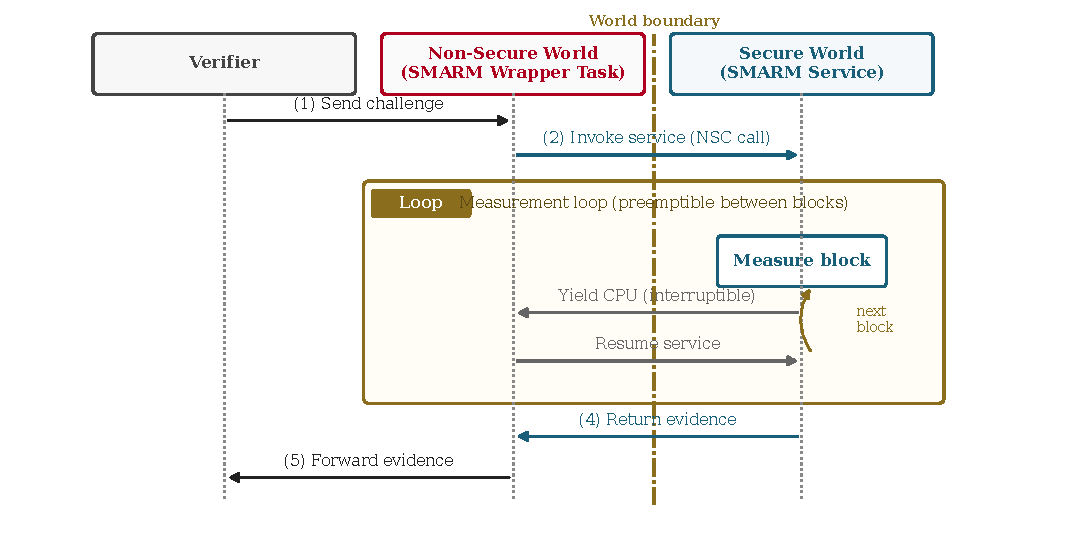
\includegraphics[width=0.92\linewidth]{smarm_workflow.pdf}
  \caption{End-to-end workflow of the TrustZone-M-based SMARM
    realization. Real-time tasks may preempt the Wrapper Task
    between consecutive block measurements.}
  \label{fig:workflow}
\end{figure}
 
\subsection{Frequency Accuracy Ratio (FAR)}
 
We quantify real-time availability as:
\[
  \mathrm{FAR} = \frac{f_{\mathrm{observed}}}{f_{\mathrm{baseline}}},
\]
where $f_{\mathrm{observed}}$ is the real-time task's frequency during
attestation and $f_{\mathrm{baseline}}$ its frequency without
attestation. FAR~$= 1.0$ means no interference; lower values indicate
degradation.

% ================================================================
\section{Motivation}
\label{sec:motivation}
 
\subsection{The Non-Interruptibility Bottleneck}
 
SMARM's baseline design disables interrupts for the entire
duration of the SHA-256 hash computation over each block.
The non-interruptibility period scales linearly with block size:
\[
  t_{\mathrm{disabled}}(B) = \frac{B}{\text{SHA-256 throughput}}
  \approx \frac{B}{1.1\;\text{MB/s}}.
\]
On our target platform, this yields \tdis values from 0.062~ms
at $B = 64$~bytes up to 3.75~ms at $B = 4096$~bytes. A 1000~Hz
real-time control task has a period of 1~ms; at $B = 4096$~bytes,
a single block measurement holds interrupts disabled for $3.75\times$
the task period, causing multiple missed executions.
 
Figure~\ref{fig:timing_diagram} illustrates the fundamental
difference between traditional RA, SMARM baseline, and Atomic
Copy. Traditional RA disables interrupts for the entire
measurement (seconds). SMARM baseline reduces this to per-block
hash duration. Atomic Copy further reduces it to per-block copy
duration only.
 
\begin{figure}[!htp]
  \centering
        \centering
        \includegraphics[width=\linewidth]{timing_diagram.png}
        \label{fig:baseline_results_1000hz}
 
  \caption{Timing comparison of interrupt-disabled windows across
    attestation approaches. Traditional RA disables interrupts for
    the entire scan. SMARM limits the disabled window to per-block
    hashing. Atomic Copy further reduces it to per-block memory copy
    only, allowing the longer hash computation to execute with
    interrupts enabled.}
  \label{fig:timing_diagram}
\end{figure}
 
\subsection{FAR Degradation Under Real-Time Workloads}



\begin{figure}[!ht]
    \centering
    \begin{subfigure}[t]{\linewidth}
        \centering
        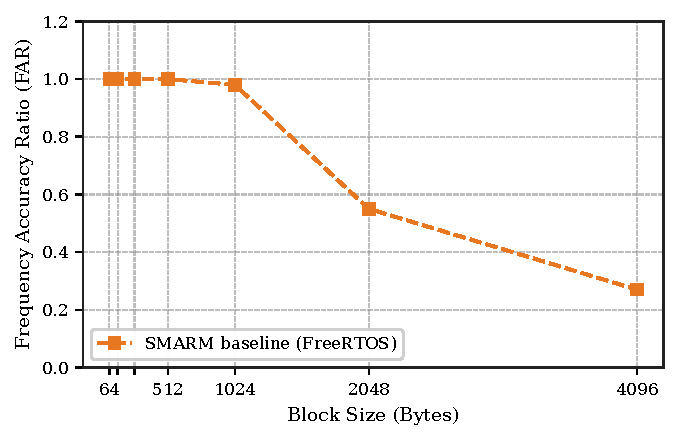
\includegraphics[width=\linewidth]{far_1000.pdf}
        \caption{High real-time workload (1000~Hz)}
        \label{fig:baseline_results_1000hz}
    \end{subfigure}
    \vspace{0.2em}
    \begin{subfigure}[t]{\linewidth}
        \centering
        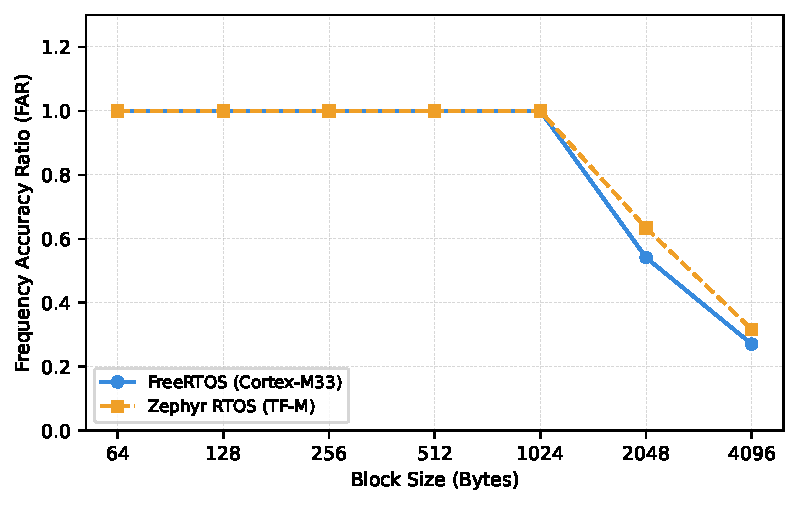
\includegraphics[width=\linewidth]{far_100.pdf}
        \caption{Medium real-time workload (100~Hz)}
        \label{fig:baseline_results_100hz}
    \end{subfigure}
    \vspace{0.6em}
    \begin{subfigure}[t]{\linewidth}
        \centering
        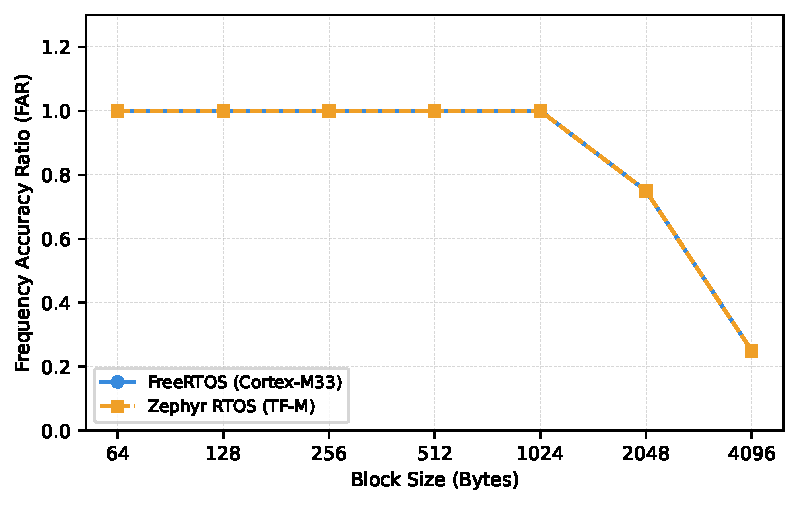
\includegraphics[width=\linewidth]{far_10.pdf}
        \caption{Low real-time workload (10~Hz)}
        \label{fig:baseline_results_10hz}
    \end{subfigure}
    \caption{Real-time availability (FAR) of SMARM under different 
    real-time workloads across block sizes and RTOS platforms. 
    FAR~$\approx 1.0$ for $B \leq 1024$~bytes across all configurations, 
    but degrades significantly at $B \geq 2048$~bytes. Both FreeRTOS and 
    Zephyr exhibit nearly identical trends across all workload classes, 
    indicating that block size rather than RTOS-specific behavior is the 
    dominant factor.}
    \label{fig:setup_and_baseline_far}
\end{figure}


Figure~\ref{fig:setup_and_baseline_far} confirms the impact. At
$B = 4096$~bytes under the 1000~Hz workload, FAR drops to
$\approx 0.27$: the real-time task runs at less than one-third
of its intended frequency. The RTOS choice (FreeRTOS vs.\ Zephyr)
has negligible effect, confirming that the interference is caused
by \smarm's per-block atomic window, not scheduling policy.

\textbf{Root cause.} The SHA-256 hash computation does not
inherently require atomicity. What must be atomic is the
\emph{capture} of the block's contents: if malware modifies the
block mid-hash, the measurement is corrupted. However, if a
snapshot is first taken atomically into a Secure-world buffer,
hashing can then proceed on the snapshot with interrupts enabled.
Since memory copy on Cortex-M33 runs at $\approx 17$~MB/s versus
$\approx 1.1$~MB/s for SHA-256, this decoupling reduces \tdis
by approximately $15\times$.

% ================================================================
\section{Atomic Copy Enhancement}
\label{sec:design}
 
\subsection{Key Insight and Workflow}
 
We redesign the Secure Service so that each block measurement
comprises two distinct phases:
\begin{enumerate}
  \item \textbf{Atomic copy} (interrupts \emph{disabled}):
    capture a snapshot of $M_{\sigma(i)}$ into a Secure-world
    buffer via \texttt{Memcpy}. This window is
    $t_{\mathrm{disabled}}^{\mathrm{copy}} = B /
    17\,\text{MB/s}$.
  \item \textbf{Hash computation} (interrupts \emph{enabled}):
    invoke \texttt{HMAC.Update} on the captured snapshot.
    Real-time tasks may preempt here.
\end{enumerate}
 
Figure~\ref{fig:atomic_workflow} shows the end-to-end workflow.
The structure is identical to baseline SMARM except that
Phase~2 of each iteration is split into an atomic copy followed
by an interrupt-enabled hash.
 
\begin{figure}[!ht]
    \centering
    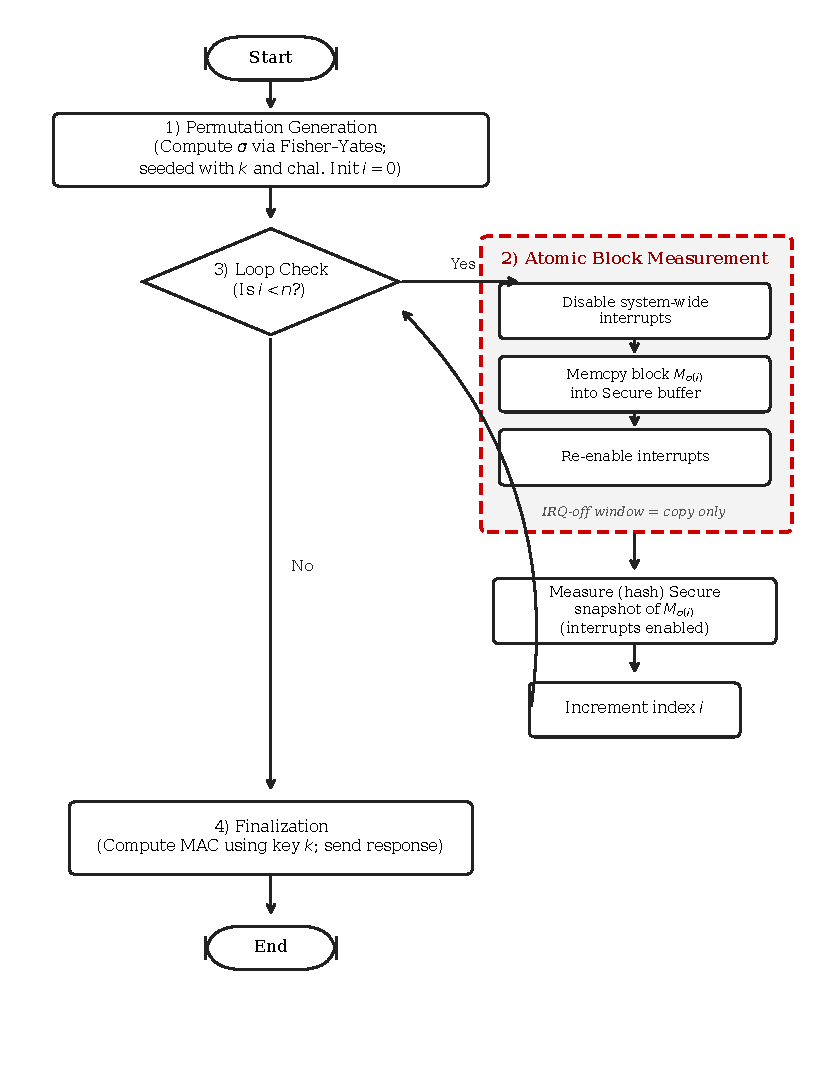
\includegraphics[width=\linewidth]{atomic_workflow.pdf}
    \caption{End-to-end workflow of the atomic copy enhancement. 
    Each iteration consists of two phases: an \emph{atomic copy} step 
    (interrupts disabled) that captures a snapshot of the memory block 
    into a Secure-world buffer, followed by a \emph{hash computation} 
    step (interrupts enabled) over the captured snapshot. Compared to 
    the SMARM baseline (Figure~\ref{fig:smarm_workflow}), the 
    interrupt-disabled window per block is reduced from 
    $t^{\mathrm{hash}}_{\mathrm{disabled}}$ to 
    $t^{\mathrm{copy}}_{\mathrm{disabled}}$, where 
    $t^{\mathrm{copy}}_{\mathrm{disabled}} \ll 
    t^{\mathrm{hash}}_{\mathrm{disabled}}$.}
    \label{fig:atomic_copy_workflow}
\end{figure}

\subsection{Protocol}

Algorithm~\ref{alg:atomic_copy} specifies the enhanced Secure Service.
The only structural change from baseline SMARM is the insertion of an
atomic copy step before each HMAC update (lines 5--7), after which
interrupts are immediately re-enabled and hashing proceeds on the
captured buffer.

\begin{algorithm}[!ht]
\caption{Atomic Copy Secure Service}
\label{alg:atomic_copy}
\begin{algorithmic}[1]
\Require $n$ blocks, shuffled indices $\sigma$, memory $M$, key $k$
\State \Call{HMAC.Init}{$k$}
\For{$i \gets 0$ to $n-1$}
  \State $\mathit{blk} \gets M[\sigma(i) \cdot B]$
  \State \Call{DisableInterrupts}{}
  \State \Call{Memcpy}{\textit{buf}, \textit{blk}, $B$} \Comment{atomic snapshot}
  \State \Call{EnableInterrupts}{}
  \State \Call{HMAC.Update}{\textit{buf}, $B$} \Comment{interrupts on}
\EndFor
\State \textbf{return} \Call{HMAC.Finalize}{}
\end{algorithmic}
\end{algorithm}

\subsection{Security Argument}
 
Atomic Copy preserves all three of SMARM's security requirements:
 
\textbf{(S1) Controlled Execution.} The Secure Service remains
accessible only via TrustZone-M NSC entry points. Interrupts are
disabled \emph{throughout} \texttt{Memcpy}, preventing malware from
modifying the source block between the start and end of the copy.
If an interrupt occurred mid-copy, the Secure-world buffer could
capture a partially modified block; disabling interrupts during the
entire copy prevents this race condition. The atomicity invariant
is preserved — only the protected operation has shifted from
hashing to copying.
 
\textbf{(S2) Key Secrecy.} The attestation key $k$ and all
HMAC state reside exclusively in Secure RAM throughout.
Atomic Copy does not modify the storage or usage of $k$.
 
\textbf{(S3) Private Measurement Order.} The permutation $\sigma$
continues to reside in Secure RAM and is not exposed to the
Non-Secure world. Atomic Copy does not alter permutation
generation or storage.
 
Subsequent hash computation operates on the captured buffer in
Secure RAM, which is inaccessible to Non-Secure code regardless
of interrupt state.

% ================================================================
\section{Evaluation}
\label{sec:eval}

\subsection{Setup}

We evaluate on the STM32L552ZE Nucleo-144 board (ARM Cortex-M33
at 110~MHz) running FreeRTOS. Block sizes
$B \in \{64, 128, 256, 512, 1024, 2048, 4096\}$~bytes are evaluated
over 512~KB of attested memory. We measure:
\begin{itemize}
  \item \tdis using the on-chip TIM2 timer (137.5~kHz,
    7.27~$\mu$s resolution), averaged over 5 rounds.
  \item \FAR under high (1000~Hz), medium (100~Hz), and low (10~Hz)
    real-time workloads, using the same protocol as
    Section~\ref{sec:motivation}.
\end{itemize}

\subsection{Non-Interruptibility Period}

\begin{table}[!ht]
  \centering
  \small
  \caption{$t_{\mathrm{disabled}}$ comparison: SMARM baseline vs.\
    Atomic Copy on STM32L552ZE running FreeRTOS. Values averaged
    over 5 rounds; std.\ dev.\ $< 0.003$~ms in all cases.}
  \label{tab:tdisabled}
  \setlength{\tabcolsep}{4pt}
  \begin{tabular}{rrrrr}
    \toprule
    & \multicolumn{2}{c}{\textbf{SMARM Baseline}} 
    & \multicolumn{2}{c}{\textbf{Atomic Copy}} \\
    \cmidrule(lr){2-3}\cmidrule(lr){4-5}
    \textbf{$B$ (bytes)} & Mean (ms) & Std & Mean (ms) & Std \\
    \midrule
    64   & 0.062 & 0.001 & $<$0.007$^\dagger$ & --- \\
    128  & 0.120 & 0.001 & 0.008 & 0.001 \\
    256  & 0.237 & 0.001 & 0.015 & 0.001 \\
    512  & 0.472 & 0.002 & 0.031 & 0.001 \\
    1024 & 0.939 & 0.001 & 0.060 & 0.001 \\
    2048 & 1.877 & 0.003 & 0.119 & 0.003 \\
    4096 & 3.749 & 0.002 & 0.243 & 0.001 \\
    \bottomrule
  \end{tabular}

  \smallskip
  \raggedright\footnotesize
  $^\dagger$At $B = 64$~bytes, Atomic Copy completes within one TIM2
  tick ($7.27\,\mu$s); we report an upper bound.
  The reduction relative to baseline is $\geq 9\times$ at this size.
\end{table}

Table~\ref{tab:tdisabled} shows that Atomic Copy consistently reduces
\tdis by $15$--$16\times$ for $B \geq 128$~bytes, reflecting the
throughput ratio between memory copy ($\approx 17$~MB/s) and
SHA-256 ($\approx 1.1$~MB/s) on Cortex-M33.






\subsection{Real-Time Availability}


\begin{figure}[!ht]
\centering
\begin{subfigure}[t]{\linewidth}
    \centering
    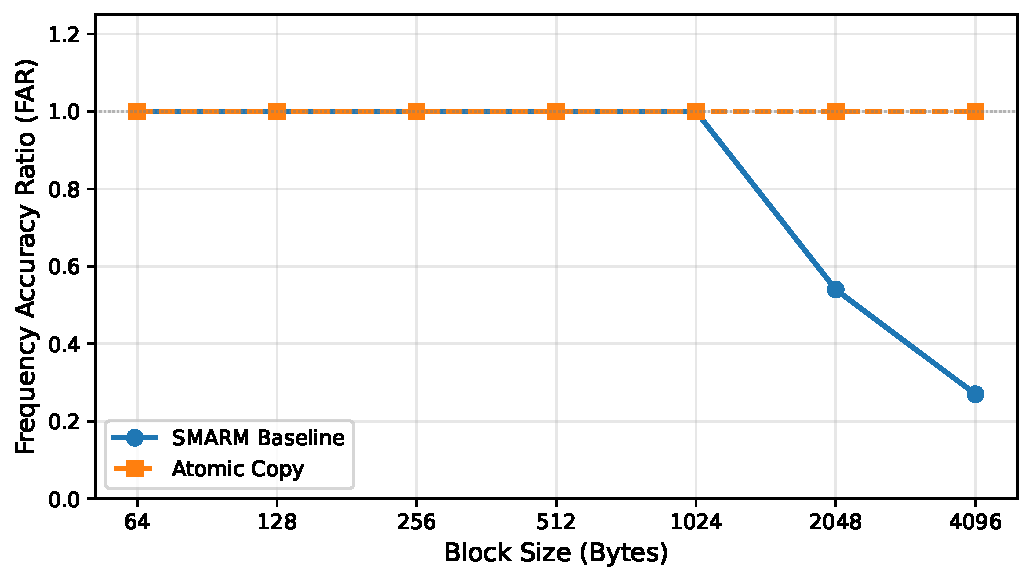
\includegraphics[width=\linewidth]{far_atomic_1000hz.pdf}
    \caption{High real-time workload (1000~Hz)}
    \label{fig:far_atomic_1000}
\end{subfigure}
\vspace{0.5em}
\begin{subfigure}[t]{\linewidth}
    \centering
    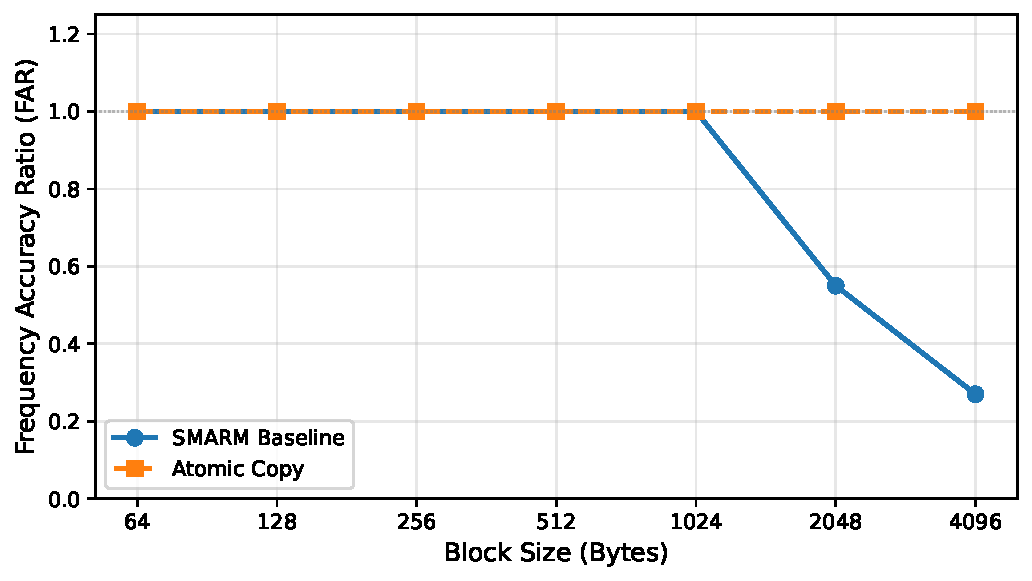
\includegraphics[width=\linewidth]{far_atomic_100hz.pdf}
    \caption{Medium real-time workload (100~Hz)}
    \label{fig:far_atomic_100}
\end{subfigure}
\vspace{0.5em}
\begin{subfigure}[t]{\linewidth}
    \centering
    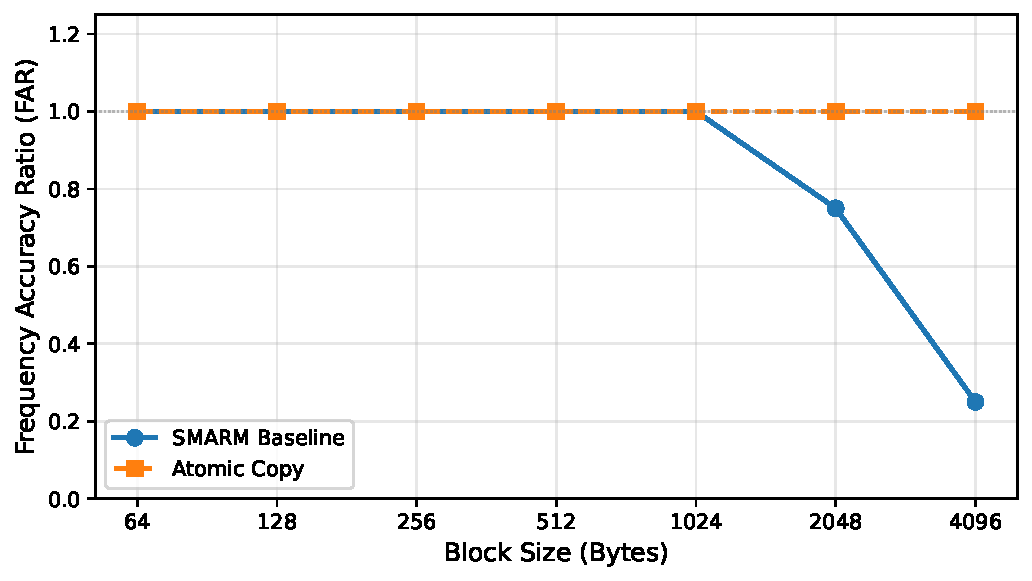
\includegraphics[width=\linewidth]{far_atomic_10hz.pdf}
    \caption{Low real-time workload (10~Hz)}
    \label{fig:far_atomic_10}
\end{subfigure}
\caption{Real-time availability (FAR) of the atomic copy 
enhancement compared to SMARM baseline across block sizes and 
real-time workload classes on STM32L552ZE running FreeRTOS. The 
atomic copy variant maintains FAR~$\approx 1.0$ across all block 
sizes up to 4096 bytes, while the baseline degrades sharply at 
$B \geq 2048$ bytes.}
\label{fig:far_atomic}
\end{figure}


Figure~\ref{fig:far_atomic} presents the key result. Atomic Copy
maintains FAR~$= 1.0$ across \emph{all} evaluated block sizes and
all three workload classes, including $B \in \{2048, 4096\}$~bytes
where the SMARM baseline degrades significantly. At $B = 4096$~bytes
under the 1000~Hz workload, SMARM baseline achieves FAR~$\approx 0.27$
while Atomic Copy achieves FAR~$\approx 1.0$ — a complete
elimination of real-time interference.

\textbf{Interpretation.} At $B = 4096$~bytes, the SMARM baseline
disables interrupts for $3.75$~ms per block, exceeding the $1$~ms
period of a 1000~Hz task nearly $4\times$. The real-time task misses
multiple execution slots per block measurement. With Atomic Copy,
the disabled window shrinks to $0.243$~ms — well below the task
period — and the task preempts freely during the subsequent
interrupt-enabled hash computation.

\subsection{Storage Overhead}

Atomic Copy introduces one additional Secure-world buffer of size
$B$~bytes. On our target platform, this ranges from 64~bytes at
$B = 64$~bytes to 4096~bytes at $B = 4096$~bytes. At the real-time
boundary block size ($B = 1024$~bytes), the buffer adds 1024~bytes
to the Secure RAM usage, on top of the permutation $\sigma$
(576~bytes). The total Secure RAM footprint at $B = 1024$~bytes
increases from 576~bytes (baseline) to 1600~bytes (Atomic Copy) —
still well within the 128~KB Secure RAM budget of the STM32L552ZE.

% ================================================================
\section{Related Work}
\label{sec:related}
 
\textbf{Traditional RA.} SMART~\cite{eldefrawy2012smart},
VRASED~\cite{nunes2019vrased}, and HYDRA~\cite{eldefrawy2017hydra}
require atomic execution of the entire memory measurement, with
VRASED disabling interrupts for up to 0.45~s, making them
incompatible with real-time workloads.
 
\textbf{Shuffled measurement.}
SMARM~\cite{carpent2018smarm} reduces the atomic window to a
single block. PRoM~\cite{aman2021prom} extends this to multi-core
devices; HAtt~\cite{aman2018hatt} combines PUFs with shuffled
measurement. ITERATOR~\cite{sponziello2025iterator} uses Cuckoo
filters for storage efficiency. None of these works have been
evaluated under RTOS real-time workloads, and all retain per-block
atomicity over the hash computation.
 
\textbf{Interruptible attestation.}
ISC-FLAT~\cite{isc-flat} handles interrupts during \emph{control-flow}
attestation via TrustZone-M. ASAP~\cite{asap} allows selected
trusted ISRs during proof-of-execution. IDA~\cite{ida2024} supports
interrupts in hybrid attestation. These schemes target control-flow
rather than memory-content integrity and are complementary to our
approach.
 
\textbf{Hardware-assisted.}
LO-FAT~\cite{lo-fat}, LiteHAX~\cite{litehax}, and
ATRIUM~\cite{atrium} use dedicated hardware modifications to
eliminate non-interruptible windows. Our approach achieves
real-time compatibility on unmodified, off-the-shelf TrustZone-M
MCUs.
 
% ================================================================
\section{Conclusion}
\label{sec:conclusion}
 
We showed that SMARM's real-time availability degrades at block
sizes $B \geq 2048$~bytes because interrupts remain disabled for
the entire SHA-256 hash computation per block. We proposed Atomic
Copy, which shifts the atomic window from hashing to memory copy,
reducing \tdis by 15--71$\times$ across all evaluated block sizes.
Implemented on STM32L552ZE running FreeRTOS, Atomic Copy restores
FAR~$\approx 1.0$ at all block sizes up to 4096~bytes, with only a
modest increase in Secure RAM usage (at most 4208~bytes at
$B = 4096$~bytes). Atomic Copy is orthogonal to storage-reduction
techniques such as SMARM+PRNG and SMARM+FPE, and can be combined
with them to achieve both real-time compatibility and reduced secure
storage on resource-constrained TrustZone-M devices.
 
\bibliographystyle{IEEEtran}
\bibliography{citation}
 
\end{document}